\documentclass[11pt,a4paper]{article}
\usepackage[margin=2.3cm]{geometry}
\usepackage{amsmath,amssymb}
\usepackage{booktabs}
\usepackage{siunitx}
\usepackage{pgfplots}
\pgfplotsset{compat=1.17}
\usepackage[colorlinks=true,linkcolor=blue!50!black,urlcolor=blue!50!black]{hyperref}

\newcommand{\rwin}{R_{\mathrm{win}}}
\newcommand{\Ahat}{\hat{A}}
\newcommand{\code}[1]{\texttt{#1}}

\title{Inductive RF antenna in LePIC:\\ the \code{Planar} and \code{Coil} modes}
\author{LePIC modular edition --- antenna models note}
\date{\today}

\begin{document}
\maketitle

\begin{abstract}
LePIC has two prescribed-field models of a flat inductive antenna placed
behind a dielectric window. They share the window position, the plasma
shielding factor, the skin-depth update and the power controller. They differ
in where the field's spatial shape comes from. \code{Planar} uses a one-line
analytic formula with a single parameter, the window radius $\rwin$. It
supplies an electric field only. \code{Coil} computes the vacuum vector
potential of the actual coil turns. It derives both $E_\theta$ and the RF
magnetic field $\mathbf{B}_{\mathrm{RF}}$ from that potential, so the two
satisfy Faraday's law, and particles feel the $\mathbf{v}\times\mathbf{B}_{\mathrm{RF}}$ force. This note
describes both models, compares their vacuum profiles for the test cases
\code{Cyl\_planar\_RFant} and \code{Cyl\_coil\_RFant}, and lists the
differences the comparison runs can detect.
\end{abstract}

%======================================================================
\section{Common framework}
%======================================================================

\paragraph{Geometry.} The chamber is a cylinder whose axis is the $x$ axis
through the centre of the $y$--$z$ cross-section. The local radius and angle
are
\begin{equation}
  r = \sqrt{(y-y_{\max}/2)^2 + (z-z_{\max}/2)^2}, \qquad
  \theta = \operatorname{atan2}\!\left(z-z_{\max}/2,\; y-y_{\max}/2\right).
\end{equation}
The dielectric window lies at $x = x_0$ (\code{xl\_pow}), and the plasma
occupies $x > x_0$. In both modes the RF electric field is purely azimuthal:
\begin{equation}
  E_y = -E_\theta \sin\theta, \qquad E_z = E_\theta \cos\theta .
\end{equation}
It is added to the electrostatic field at each particle when the particle is
pushed. It is not deposited on the grid, and Poisson's equation does not see
it.

\paragraph{Plasma shielding.} The plasma screens the induced field over a
skin depth $\delta$. Both modes model this with the same assumed axial factor
\begin{equation}
  g(x) = \exp\!\left[-(x-x_0)/\delta\right], \qquad x > x_0 .
  \label{eq:g}
\end{equation}
Every RF period ($n_{\mathrm{RF}} = 1/(f_0\,\Delta t)$ steps), $\delta$ is
set to the collisionless skin depth of the mean electron density
$\langle n_e\rangle$ inside the window disk $r \le \rwin$, averaged over the
whole heating slab:
\begin{equation}
  \delta = \frac{c}{\omega_{pe}}, \qquad
  \omega_{pe}^2 = \frac{\langle n_e\rangle e^2}{\varepsilon_0 m_e} .
\end{equation}
Here $\varepsilon_0$ is the true value; the $k_{\varepsilon_0}$ rescaling is
undone. In the \code{Coil} mode $\rwin$ is used \emph{only} to choose this
averaging disk, so that both runs compute $\delta$ identically.

\paragraph{Absorbed power and controller.} The mover accumulates the work done
by the RF field on every macroparticle, $P_{\mathrm{RF}} = \sum_p N_m q\,
E_\theta v_\theta$, averaged over one RF period. At the end of the period the
drive amplitude $\mathcal{D}$ is rescaled towards the target $P_{\mathrm{abs}}$:
\begin{equation}
  \mathcal{D} \leftarrow \mathcal{D}\,\sqrt{P_{\mathrm{abs}}/P_{\mathrm{RF}}} .
  \label{eq:ctrl}
\end{equation}
The square root reflects $P \propto \mathcal{D}^2$ at fixed plasma. The only
difference between the modes is what $\mathcal{D}$ represents. In
\code{Planar} it is a field amplitude $E_0$ in \si{V/m}. In \code{Coil} it is
the coil current $I$ in amperes. Both are stored in the same variable
(\code{cfg\%E0\_RF}) and read from the same position in
\code{conditions.inp}.

%======================================================================
\section{\texttt{Planar}: analytic field}
%======================================================================

The field is
\begin{equation}
  E_\theta(r,x,t) = E_0\, f(r)\, g(x)\, \cos\omega t, \qquad
  f(r) =
  \begin{cases}
    r/\rwin, & r \le \rwin,\\[2pt]
    \rwin/r, & r > \rwin.
  \end{cases}
  \label{eq:planar}
\end{equation}
This $f(r)$ is the Faraday's-law field of a \emph{spatially uniform}
oscillating $B_x$ confined to the disk $r\le\rwin$. Inside the disk,
$\oint \mathbf{E}\cdot d\boldsymbol{\ell} = -\dot\Phi$ gives
$E_\theta \propto r$; outside, the enclosed flux is constant, so
$E_\theta \propto 1/r$. The profile is continuous at $\rwin$ and peaks
there.

Properties:
\begin{itemize}
  \item \textbf{Electric field only.} The implied $B_x$ is not applied to
        particles, so species keep their usual mover (the electrostatic
        mover unless a static magnetic map is loaded).
  \item \textbf{Single shape parameter $\rwin$.} The coil's actual turns,
        spacing and distance from the window do not appear. The field is a
        ring peaked exactly at $\rwin$, with a kink in its slope there.
  \item \textbf{Axial decay from shielding only.} In vacuum ($g=1$) the field
        would not decay at all along $x$. The only axial decay is
        \eqref{eq:g}.
\end{itemize}
Implementation: \code{compute\_rf\_field} in
\code{modules/particles/mod\_particleMover.f90}.

%======================================================================
\section{\texttt{Coil}: field of the actual coil turns}
%======================================================================

\paragraph{Vacuum potential.} The coil is a set of $N$ coaxial circular loops
read from \code{input\_dir/coil.inp}. Turn $j$ has radius $a_j$, axial
position $x_j$ (behind the window, $x_j < x_0$) and relative current $w_j$
($w_j = 1$ for a series coil). The vector potential of a unit-current loop
is the closed form (Jackson, 3rd ed., eq.~5.37):
\begin{equation}
  A_{\mathrm{loop}}(r,x;a,x_j) = \frac{\mu_0}{\pi k}\sqrt{\frac{a}{r}}
  \left[\left(1-\tfrac{k^2}{2}\right)K(k) - E(k)\right], \qquad
  k^2 = \frac{4ar}{(a+r)^2 + (x-x_j)^2},
\end{equation}
where $K$ and $E$ are the complete elliptic integrals. The code evaluates
them by the arithmetic--geometric mean, and switches to the series form for
$k^2 < 10^{-3}$ to avoid cancellation. At start-up the sum over turns is
tabulated once, per ampere, on an $(r,x)$ grid at half the PIC cell size:
\begin{equation}
  \Ahat(r,x) = \sum_{j=1}^{N} w_j\, A_{\mathrm{loop}}(r,x;a_j,x_j)
  \quad [\si{T.m/A}] .
\end{equation}

\paragraph{Vacuum magnetic field.} $\hat{\mathbf{B}} =
\nabla\times(\Ahat\,\hat{\boldsymbol\theta})$ is obtained by central
differences of the flux function $\psi = r\Ahat$:
\begin{equation}
  \hat B_r = -\frac{1}{r}\frac{\partial\psi}{\partial x}, \qquad
  \hat B_x = \frac{1}{r}\frac{\partial\psi}{\partial r}, \qquad
  \hat B_x(0,x) = \lim_{r\to 0}\frac{2\psi}{r^2}.
\end{equation}
Using the same central operators, the discrete $\nabla\cdot\hat{\mathbf B}$
vanishes to round-off. The start-up self-check finds about $10^{-17}$, an
on-axis error relative to the exact loop formula of about $10^{-3}$
($O(\Delta r^2)$), and the correct far-field dipole limit. The table is
written to \code{Output/coil\_field.dat}.

\paragraph{Shielding and fields applied to particles.} The same factor $g(x)$
multiplies the potential, $A = g\Ahat$. The magnetic field is then
\emph{re-derived} from the shielded potential, so it remains a curl:
\begin{equation}
  \nabla\times(g\Ahat\,\hat{\boldsymbol\theta}) :\quad
  B_r = g\left(\hat B_r + \frac{\Ahat}{\delta}\right), \qquad
  B_x = g\,\hat B_x .
\end{equation}
The extra term $\Ahat/\delta$ comes from $\partial g/\partial x$. With
$\mathbf{A}(t) = I\,A\,\hat{\boldsymbol\theta}\cos\omega t$ and $\mathbf E =
-\partial_t \mathbf A$, the particles feel
\begin{equation}
  E_\theta = \omega I\, g(x)\,\Ahat(r,x)\,\sin\omega t, \qquad
  \mathbf{B}_{\mathrm{RF}} = I\left(B_r\,\hat{\mathbf r} + B_x\,\hat{\mathbf x}\right)\cos\omega t .
  \label{eq:coil}
\end{equation}
Both fields come from the same potential, so Faraday's law
$\nabla\times\mathbf E = -\partial_t\mathbf B_{\mathrm{RF}}$ holds exactly in
the model.

\paragraph{Mover.} Because $\mathbf{B}_{\mathrm{RF}}$ needs the magnetic
rotation, the \code{Coil} mode sends \emph{every} species through the Boris
mover, with $\mathbf{B}_{\mathrm{RF}}$ added to any static field $\mathbf{B}_0$
(or used alone when $\mathbf B_0 = 0$). The energy-conserving (EC-PIC)
gather of the electrostatic field is kept, so the numerics are the same as in
\code{Planar} apart from the rotation.

Implementation: \code{modules/fields/mod\_coilField.f90} (table, evaluation,
self-check) and \code{compute\_coil\_field} /
\code{move\_and\_bc\_boris} in \code{mod\_particleMover.f90}.

%======================================================================
\section{Side-by-side summary}
%======================================================================

\begin{center}
\renewcommand{\arraystretch}{1.25}
\begin{tabular}{@{}p{0.27\textwidth}p{0.33\textwidth}p{0.33\textwidth}@{}}
\toprule
 & \code{Planar} & \code{Coil} \\
\midrule
Source of the shape & formula \eqref{eq:planar}, one parameter $\rwin$
  & vacuum $\Ahat(r,x)$ of the turns in \code{coil.inp} \\
Radial profile & $r/\rwin$ then $\rwin/r$; sharp peak at $\rwin$
  & smooth; set by turn radii and their distance to the window \\
Axial decay & $g(x)$ only
  & vacuum decay of $\Ahat$ \emph{times} $g(x)$ \\
RF magnetic field & none (implied $B_x$ not used)
  & $B_r$, $B_x$ from $\nabla\times(g\Ahat\hat{\boldsymbol\theta})$ \\
Faraday's law & not enforced (no $\mathbf B$)
  & exact within the model \\
Particle mover & unchanged (electrostatic)
  & Boris for all species, $\mathbf B_0 + \mathbf B_{\mathrm{RF}}$ \\
Controlled amplitude & $E_0$ [\si{V/m}] & coil current $I$ [\si{A}] \\
Time phase of $E_\theta$ & $\cos\omega t$ & $\sin\omega t$ ($\mathbf B\propto\cos\omega t$) \\
Role of $\rwin$ & field shape \emph{and} $\langle n_e\rangle$ disk
  & $\langle n_e\rangle$ disk only \\
Shared & \multicolumn{2}{p{0.66\textwidth}}{window $x_0$, factor $g(x)$, $\delta = c/\omega_{pe}$ update every RF period,
  controller \eqref{eq:ctrl}, power diagnostic $\sum N_m q E_\theta v_\theta$} \\
\bottomrule
\end{tabular}
\end{center}

%======================================================================
\section{Vacuum profiles for the comparison cases}
%======================================================================

The two cases are identical except for the RF mode: Ar at \SI{1}{Pa},
cylinder of radius $R = \SI{5}{cm}$ and length \SI{10}{cm}, $80^3$ cells,
$n_0 = \SI{5e16}{m^{-3}}$, $f_0 = \SI{13.56}{MHz}$,
$P_{\mathrm{abs}} = \SI{15}{W}$, $\rwin = \SI{4}{cm}$. The coil has four
turns, $a_j = 1,2,3,4$~cm, all at $x_j = -0.5$~cm (\SI{5}{mm} behind the
window), in series. The curves below are computed from the formulas above,
with the same loop formula and turns as the code.

\begin{figure}[ht]
\centering
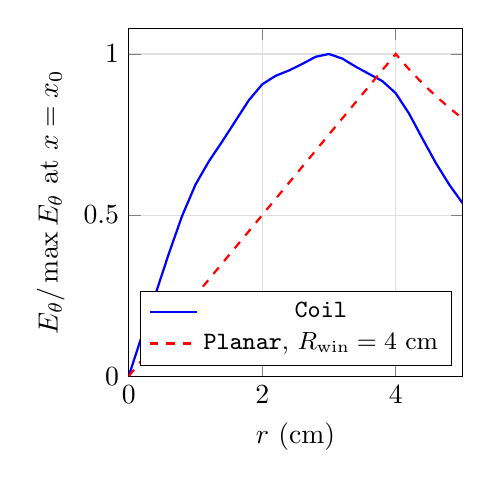
\begin{tikzpicture}
\begin{axis}[
  width=0.48\textwidth, height=6cm,
  xlabel={$r$ (cm)}, ylabel={$E_\theta / \max E_\theta$ at $x=x_0$},
  xmin=0, xmax=5, ymin=0, ymax=1.08,
  legend pos=south east, legend style={font=\small},
  grid=major, grid style={gray!25}]
\addplot[thick, blue] coordinates {
(0.0,0.0000)(0.2,0.1267)(0.4,0.2537)(0.6,0.3796)(0.8,0.4974)(1.0,0.5944)
(1.2,0.6664)(1.4,0.7282)(1.6,0.7924)(1.8,0.8565)(2.0,0.9058)(2.2,0.9322)
(2.4,0.9488)(2.6,0.9691)(2.8,0.9913)(3.0,1.0000)(3.2,0.9858)(3.4,0.9607)
(3.6,0.9381)(3.8,0.9159)(4.0,0.8783)(4.2,0.8150)(4.4,0.7376)(4.6,0.6621)
(4.8,0.5951)(5.0,0.5373)};
\addlegendentry{\code{Coil}}
\addplot[thick, red, dashed] coordinates {
(0.0,0.0)(4.0,1.0)(4.2,0.9524)(4.4,0.9091)(4.6,0.8696)(4.8,0.8333)(5.0,0.8000)};
\addlegendentry{\code{Planar}, $\rwin=4$ cm}
\end{axis}
\end{tikzpicture}
\hfill
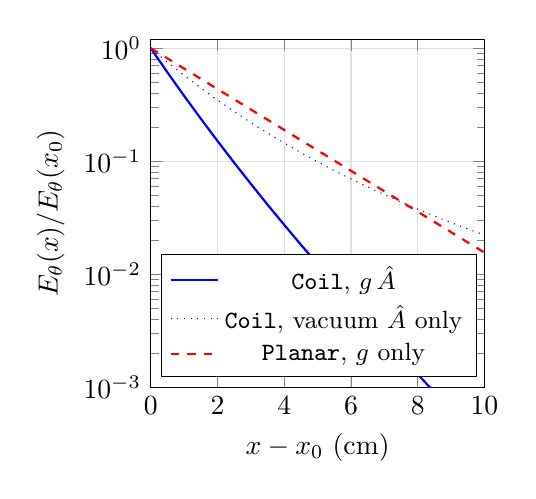
\begin{tikzpicture}
\begin{axis}[
  width=0.48\textwidth, height=6cm,
  xlabel={$x - x_0$ (cm)}, ylabel={$E_\theta(x)/E_\theta(x_0)$},
  xmin=0, xmax=10, ymode=log, ymin=1e-3, ymax=1.2,
  legend pos=south west, legend style={font=\small},
  grid=major, grid style={gray!25}]
\addplot[thick, blue] coordinates {
(0.0,1.0000)(0.5,0.6099)(1.0,0.3786)(1.5,0.2377)(2.0,0.1509)(2.5,0.0969)
(3.0,0.0629)(3.5,0.0412)(4.0,0.0273)(4.5,0.0182)(5.0,0.0123)(5.5,0.0083)
(6.0,0.0057)(6.5,0.0039)(7.0,0.0027)(7.5,0.0019)(8.0,0.0013)(8.5,0.0009)
(9.0,0.0007)(9.5,0.0005)(10.0,0.0003)};
\addlegendentry{\code{Coil}, $g\,\Ahat$}
\addplot[thin, blue, dotted] coordinates {
(0.0,1.0000)(0.5,0.7512)(1.0,0.5743)(1.5,0.4441)(2.0,0.3473)(2.5,0.2747)
(3.0,0.2195)(3.5,0.1773)(4.0,0.1445)(4.5,0.1189)(5.0,0.0987)(5.5,0.0825)
(6.0,0.0696)(6.5,0.0591)(7.0,0.0505)(7.5,0.0434)(8.0,0.0376)(8.5,0.0327)
(9.0,0.0286)(9.5,0.0251)(10.0,0.0222)};
\addlegendentry{\code{Coil}, vacuum $\Ahat$ only}
\addplot[thick, red, dashed, domain=0:10, samples=41] {exp(-x/2.4)};
\addlegendentry{\code{Planar}, $g$ only}
\end{axis}
\end{tikzpicture}
\caption{Vacuum shape of $E_\theta$ for the comparison cases.
Left: radial profile at the window. Right: axial profile at $r = 3$~cm (the
\code{Coil} peak), with $\delta = \SI{2.4}{cm}$, the value both runs hold.}
\label{fig:profiles}
\end{figure}

The main quantitative differences are:
\begin{enumerate}
  \item \textbf{Radial.} The \code{Coil} field peaks at $r \approx 3$~cm, not
        4~cm, and is much broader. It reaches 60\% of its peak at $r=1$~cm,
        where \code{Planar} is at 25\%. It is weaker near the side wall: 54\%
        of peak at $r=R=5$~cm, against 80\% for \code{Planar}.
  \item \textbf{Axial.} Without shielding, $\Ahat$ already falls to $1/e$ at
        $\SI{1.9}{cm}$ from the window. Combined with $g$, the effective
        $e$-folding length is about
        $(1/1.9 + 1/2.4)^{-1} \approx \SI{1.1}{cm}$, roughly half of
        \code{Planar}'s $\delta = \SI{2.4}{cm}$. At $x-x_0 = 1$~cm the
        \code{Coil} field is 38\% of its window value, against 66\% for
        \code{Planar}. The \code{Coil} power is therefore deposited in a much
        thinner layer next to the window.
  \item \textbf{Amplitude per ampere.} At the window, the peak field is
        $\omega\Ahat_{\max} \approx \SI{73}{V/m}$ per ampere at
        \SI{13.56}{MHz} (before shielding). For comparison, the
        \code{Planar} run settled at $E_0 \approx \SI{266}{V/m}$. Because the
        \code{Coil} heating volume is smaller, matching \SI{15}{W} will likely
        need a peak field of the same order or larger, so the converged
        current should be a few amperes. The \SI{1.5}{A} starting guess is
        expected to be revised upwards.
  \item \textbf{RF magnetic field.} On axis at the window,
        $\hat B_x \approx \SI{1.1e-4}{T/A}$ (\SI{1.1}{G/A}). For
        $I \sim$ \SIrange{1.5}{4}{A}, $|\mathbf B_{\mathrm{RF}}| \sim$
        \SIrange{1.6}{4.4}{G}, which gives
        $f_{ce} \approx$ \SIrange{4.6}{12}{MHz}, below or close to $f_0$.
        The magnetic force is not negligible near the window. It is absent
        from \code{Planar}.
\end{enumerate}

%======================================================================
\section{What the comparison tests}
%======================================================================

Both modes \emph{prescribe} the field, using the same assumed shielding
$g(x)$ and the same $\delta$. Neither solves the inductive (Maxwell) problem
with the plasma current. The two runs therefore isolate two questions:
\begin{itemize}
  \item whether the plasma is sensitive to the \emph{spatial shape} of the
        heating (a ring at 4~cm with 2.4~cm decay, or a broad profile with
        about 1.1~cm decay), and
  \item whether the $\mathbf v\times\mathbf B_{\mathrm{RF}}$ force has an
        effect.
\end{itemize}
The diagnostics to compare are $T_e$, the $n_e$ profile and its peaking,
$\delta(t)$ (\code{Output/skin\_depth.dat}), the converged drive amplitude,
the electron and ion wall energies $E_{k,w}$, and the power split
$P_{\mathrm{coll}}/P_{\mathrm{wall}}$ (\code{Output/Ptot.dat}). The bias
power $V_{\mathrm{bias}} |I_{\mathrm{net}}|$ is computed from the
\code{Iw*.dat} columns of grid~2.

\textbf{If the results agree} within statistical noise, the simple
\code{Planar} formula is adequate for this regime. A self-consistent 2D
inductive solve (Phase~2) is then unnecessary.
\textbf{If they differ}, the shape or the RF magnetic field matters, and
Phase~2 is justified. Phase~2 would replace the assumed $g(x)$ and the
vacuum $\Ahat$ by a solution of
$\nabla^2 \mathbf A - i\omega\mu_0\sigma\mathbf A = -\mu_0 \mathbf J_{\mathrm{coil}}$
using the PIC plasma conductivity.

\paragraph{Reference results (\code{Planar}, to 34~\textmu s).}
\begin{itemize}
  \item $E_0$ converged to \SI{266}{V/m}, and $P_{\mathrm{RF}} =
        \SI{15.00 \pm 0.05}{W}$ from \SI{0.5}{\micro s} onwards.
        $\delta = $ \SIrange{2.37}{2.40}{cm}.
  \item $P_{\mathrm{wall}} \approx \SI{-8.4}{W}$ and
        $P_{\mathrm{coll}} \approx \SI{-13.5}{W}$.
  \item $E_{k,w}(e) \approx \SI{4.9}{eV}$ and
        $E_{k,w}(\mathrm{Ar^+}) \approx \SI{26}{eV}$.
  \item About 98\% of the electron loss goes to the \SI{+20}{V} end
        electrode. It supplies about \SI{4.8}{W}, which leaves the same
        $\approx\SI{-2}{W}$ residual as the Maxwellian-heated reference case.
\end{itemize}

\end{document}
